\documentclass[11pt]{article}
\title{MATH 222 Assignment 2}
\author{Sterling Laird - V00834995}
\date{February 7, 2019}

\usepackage{enumitem}
\usepackage{amsmath}
\usepackage{amssymb}
\usepackage {tikz}

\graphicspath{ {./} }

\setlength{\parindent}{1.7cm}

\begin{document}

\maketitle
\pagebreak

\begin{enumerate}[]
    \item
    	Consider a tree $T$ with some vertex $v$ of degree 4.\\
    	Since a tree cannot have any cycles, every path from $v$ taking a unique edge incident to $v$ must eventually terminate in at least one leaf.\\
    	Therefore $T$ must have at least 4 leaves.\\
    	Now lets consider if $T$ has another vertex $u$ of degree 3.\\
    	Since $T$ is a tree, there must be a single $v$-$u$ path in $T$.\\
    	And since there must be a single $v$-$u$ path and there can be no cycles, exactly one of the edges incident to $v$ must yield a $v$-$u$ path and exactly one of the edges incident to $u$ must yield a $u$-$v$ path.\\
    	So there are exactly 3 paths from $v$ taking a unique edge incident to $v$ that terminate in at least one leaf, and similarly  there are exactly 2 paths from $u$ taking a unique edge incident to $u$ that terminate in at least one leaf.\\
    	$\therefore$ $T$ contains at least 5 leaves.
    \item 
    	For a tree $T=(V,E)$, there must have a single $u$-$v$ path in $T$ $\forall u,v \in V$.\\
    	For a trail to be Eulerian it would need to include every vertex in $T$, including all leaves.\\
    	Since a leaf only has one edge incident to it, including a leaf in the trail (not including endpoints) would result in taking the edge twice, violating a property of an Eulerian trail.\\
    	Since leaves at the endpoints only need the adjacent edge to be traversed once, they can be in the Eulerian trail.\\
    	Similarly if $T$ only has 2 leaves, a Eulerian trail would simply be the $u-v$ path between them.\\
    	$\therefore$ $T$ has a Eulerian trail iff $T$ has exactly 2 leaves.
    \item \mbox{}
    \begin{center}
		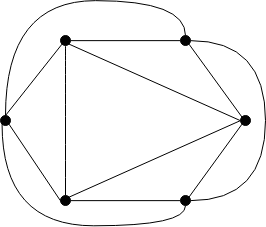
\includegraphics[scale=0.5]{q3-graph.png}\\
		Example of a 4-regular plane graph with 6 vertices.
	\end{center}
	Since $|V|-|E|+R=2 \iff 6 - 12 + 8 = 2$ holds, we can verify that this example holds.
   		
    \item
		We can use the theorem that $|E| \leq 3|V|-6$ for any planar graph $G$ with $|V| \geq 3$.\\
		Assume that both $G$ and $\overline{G}$ are planar.\\
		Therefore for $G$:
		\begin{gather}
		|E| \leq 3|V|-6 \nonumber \\
		|E| \leq 3|11|-6 \nonumber \\
		|E| \leq 27 \nonumber
		\end{gather}
		
		And therefore for $\overline{G}$, since the maximum number of edges in $\overline{G}$ is the difference between the number of edges in $K_{11}$ and the maximum number of edges in $G$ :
		\begin{gather}
		|E| \leq 3|V|-6 \nonumber \\
		\frac{11(11-1)}{2} -27 \leq 3|11|-6 \nonumber \\
		28 \leq 27 \nonumber
		\end{gather}
		Which is a contradiction.\\
		$\therefore$ either $G$ or $\overline{G}$ must be non-planar.
    \item
    	First we prove that if deg($v$) $< k$ and $G$ is k-colorable then $G-v$ is k-colorable.\\
		Since $G$ is k-colorable using Brooks' theorem, we know that the maximum degree of a vertex in $G$ must be $k-1$.\\
		Since the maximum degree of $G-v$ is less or equal the maximum degree of $G$ because some edges in $G$ may have been removed, therefore the maximum degree of $G-v$ must be $k-1$.\\
		$\therefore$ if $G$ is k-colorable, $G-v$ must be k-colorable.\\
    	Now we prove that if $G-v$ is k-colorable then $G$ is k-colorable.\\    	
    	Using Brooks's theorem the maximum degree of $G-v$ is $k-1$.\\
    	And since $v<k$, $G$ will have a maximum degree of $k$ since each of the vertices in $G-v$ will have at most one more edge in $G$.\\
		Since G has a maximum degree of $k$, using Brooks' theorem again we can easily see that $G$ will be k-colorable.\\  
		$\therefore$ $G$ is k-colorable iff $G-v$ is k-colorable.  	 
    \item
    \begin{enumerate}[label=\alph*)]
    \item
    	As a counter-example, consider $C_5$ in which $\chi(C_5) = 3$ yet contains no subgraph isomorphic to $K_3$.
    \item
    	Consider the Wheel graph $W_6$ with  $\chi(G)=4$.\\
    	\begin{center}
		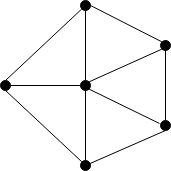
\includegraphics[scale=0.5]{q6b-graph.png}\\
		\end{center}
		While $W_6$ has a subraph homeomorphic to $K_4$, it has no subgraph isomorphic to $K_4$.\\
		$\therefore$ the statement is false.
    	
    \item
    	Since a  $\chi(G)=2$, $G$ must be bipartite.\\
    	Since for $G$ to be planar, using kuratowskis' theorem, $G$ must have no subgraph that is homeomorphic to $K_5$ or $K_{3,3}$.\\
    	Now consider $G=K_{6,6}$\\
    	We know a bipartite graph $K_{m,n}$ has a Hamiltonian cycle iff $m=n$ so $G$ has a Hamiltonian cycle.\\
    	We know that a graph with at least 2 vertices has an Eulerian circuit iff it is connected and every vertex is of even degree, so clearly $G$ has a Eulerian circuit.\\
    	Clearly $K_{3,3}$ is an isomorphic subgraph of $K_{6,6}$ so $K_{3,3}$ is a homeomorphic subgraph to $K_{6,6}$.\\
    	$\therefore$ $G=K_{6,6}$ is not planar.\\
    	$\therefore$ the statement is false
    \end{enumerate}

\end{enumerate}

\end{document}